
\chapter{Superconducting qubits and circuit quantum electrodynamics}
\label{c:scqb}

Having discussed the framework of partial, continuous, idealized quantum measurements, I will now describe the physical system we use to realize such measurements.  Rather than utilize a natural quantum system (such as an atom or single spin), we utilize engineered superconducting circuits which are described by the same quantum mechanics as natural quantum systems.  These circuit platforms have some significant advantages, especially the design flexibility in choosing various coupling strengths (created here through structures such as capacitors rather than natural dipole moments or spin-spin couplings).

\section{Quantization of electrical circuits}

The fact that electrical circuits can behave as coherent quantum variables is somehow simultaneously surprising and obvious.  It is standard practice to find a quantum description of a mechanical system by writing down the classical Lagrangian and Hamiltonian descriptions of the system, introducing commutation relations to the canonically conjugate degrees of freedom, and finally promoting these degrees of freedom to quantum operators.

For mechanical systems of rigid bodies it feels somewhat natural to consider these bodies as ``particles" and write down a quantum Hamiltonian and wavefunction for their motion, as their rigid-ness implies we can imagine all of their microscopic degrees of freedom moving together.  Of course, for large, classical objects, this description would in reality break down due to decoherence at some level. Still, experiments are continuously pushing the quantum description of mechanical rigid bodies to larger and larger objects, consisting of billions of atoms all moving together coherently in one mechanical mode \cite{Rocheleau2010,OConnell2010,Palomaki2013}.  Electrical circuits, on the other hand, consist of a large number of charge carriers, and in general there is no particular reason to believe that the quantum motion of these charge carriers should be strongly correlated to enable a similar description of their collective motion as a rigid body.

\subsection{Superconductivity}

Electrical circuits composed of superconducting materials provide a context in which it makes perfect sense to consider the motion of all of the charge carriers together as analogous to a mechanically rigid body.  Below the transition temperature in a conventional superconductor, the electrons pair to form bosonic composite particles known as Cooper pairs \cite{tinkham2004introduction}.  At very low temperature, all of these bosonic particles cool into a single collective ground state.  The excitation spectrum of the system then has a large energy gap $2 \Delta$ between the ground state and the first excited state, corresponding to the energy needed to dissociate a Cooper pair back into two electrons.

This gapped excitation spectrum is the origin of the most well known phenomenological behavior of superconductors: current flow without resistance.  The microscopic origin of resistance in a normal metal conductor is the scattering of electrons off of defects in the metal into other conduction states, corresponding to energy exchange with the lattice.  Because of the large energy gap in the spectrum of a superconductor, there are no nearby states available for Cooper pairs to scatter into, enabling the ideal flow of current without the charge carriers exchanging energy with defects in the metal.  Thus, it becomes perfectly natural to model the collective behavior of all Cooper pairs occupying the ground state as a single wavefunction.

\subsection{Quantization of an LC oscillator}

For the purposes of this thesis, a derivation of quantum circuit operators in the context of an LC oscillator will suffice.  For a more general discussion of the subject see reference \cite{Devoret1995}.

\begin{figure*}
\begin{center}
	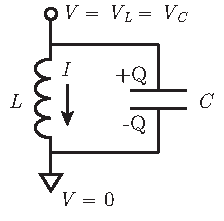
\includegraphics[width = 1.5in]{scqb_chapter/LC_osc}
\end{center}
\caption[LC oscillator circuit diagram]{LC oscillator quantities and coordinates.}
\label{fig:LC_osc}
\end{figure*}


A circuit schematic of an LC oscillator is shown in Figure \ref{fig:LC_osc}.  The classical equations of motion for an LC oscillator are usually derived using the voltage and current as the generalized coordinates.  For a quantum treatment of an LC oscillator and for quantum circuits in general it turns out to be more convenient to use the charge on the capacitor and the flux threading the inductor as the coordinates.  Fundamentally, this is because in some circuits the number of charge-carrying quanta on a metal island turns out to be a good quantum number, and in some others the total number of superconducting flux quanta threading some loop turns out to be a good quantum number.  We can write the total energy in the oscillator in the standard way as
\begin{equation}
E = \frac{1}{2} C V^2 + \frac{1}{2} L I^2.
\label{eq:LC_E}
\end{equation}
Converting to charge and flux using the relations $Q = VC$ and $\Phi = LI$, we can write the classical Hamiltonian of the LC oscillator as
\begin{equation}
H = \frac{\Phi^2}{2L} + \frac{Q^2}{2C}.
\label{eq:LC_H}
\end{equation}
Writing Hamilton's equations of motion
\begin{equation}
\frac{\partial H}{\partial \Phi} = \Phi/L = I = -\dot{Q} \quad \quad \frac{\partial H}{\partial Q} = Q/C = L\dot{I} = -\dot{\Phi}
\label{eq:LC_hams}
\end{equation}
we can immediately identify $\Phi$ as a generalized position and $Q$ as a generalized momentum, promote them to quantum operators $\hat{\Phi}$ and $\hat{Q}$, and write their commutation relation
\begin{equation}
[\hat{\Phi},\hat{Q}] = i \hbar.
\label{eq:LC_comm}
\end{equation}
Thus, the quantum dynamics of an LC oscillator are those of a quantum harmonic oscillator with raising and lowering operators $a^\dagger,a$.  We can re-express the Hamiltonian in terms of raising and lowering operators as
\begin{equation}
H = \hbar \omega a^\dagger a = \hbar \omega \hat{n}
\label{eq:LC_H_N}
\end{equation}
where $\omega = 1/\sqrt{LC}$ and $\hat{n}$ corresponds to the number operator.
States of definite energy for the system correspond to a definite number state.  Driving the LC oscillator with a classical drive at the resonant frequency results in a coherent state, where the expectation values of the quantum operators $\langle \hat{\Phi} \rangle$ and $\langle \hat{Q} \rangle$ obey the classical equations of motion and the uncertainty in the coordinate and momentum in normalized units are equal and saturate the uncertainty principle.

\section{Superconducting qubits}

An LC oscillator, when cooled to the quantum ground state and operated in a regime where there is no energy dissipation (ie when the impedance of the oscillator is purely imaginary), is a completely quantum system.  In principle, highly nonclassical states of the oscillator such as number states could be created,  but in general this requires quantum control over the degrees of freedom of the oscillator.  In other words, to prepare a nonclassical state of the oscillator, we need to couple it to some other quantum system.

We would like to be able to create highly nonclassical states of a circuit using only straightforward classical drives; however, as mentioned previously, driving an LC oscillator with a classical signal results in a coherent state of the oscillator, a highly classical state with essentially no interesting intrinsic quantum properties.  If we wanted to create, say, a state of definite excitation number (also known as a Fock state), or a explicit superposition between two of these number states, and only utilize classical controls, we need to consider a circuit with more complex dynamics than a simple harmonic oscillator.

Traditionally, superconducting qubits are introduced by discussing the Cooper pair box (aka charge qubit) and RF SQUID (aka flux qubit) circuits, as these are the simplest circuits that demonstrate behavior where the charge or flux in the circuit are a good quantum number \cite{scqubitsrev2008}.  However, modern superconducting qubits have moved away from these relatively simple and pure designs towards an intermediate regime where neither charge nor flux are good quantum numbers.  As such, I will instead introduce how to make a qubit by starting with a harmonic oscillator and introducing a weak anharmonicity rather than starting with a highly anharmonic system.

\subsection{Anharmonic oscillator as a qubit}

\begin{figure*}
\begin{center}
	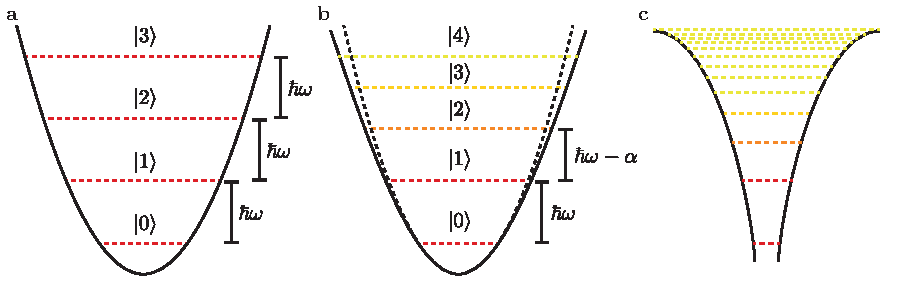
\includegraphics[width = 6in]{scqb_chapter/anharmonic_potential}
\end{center}
\caption[Harmonic and anharmonic potential energy and level spacing]{\textbf{a} Harmonic oscillator potential and energy levels, showing equal level spacing of $\hbar \omega$.  \textbf{b} Harmonic potential (dashed black line) with a softening correction (solid black line), showing decreasing energy level spacing by the anharmonicity parameter $\alpha$ with increasing energy level.  A stiffening potential would produce a positive anharmonicity rather than a negative one, increasing the frequency of higher level transitions.  \textbf{c} Rough schematic of the potential of a highly anharmonic system such as a hydrogen atom.  In general the anharmonicity in an atomic system is quite large as the potential is far removed from that of a harmonic oscillator; for the three lowest-lying states of the simple hydrogen atom, $E_{12} \approx 0.15 E_{01}$, a fractional anharmonicity of order unity.}
\label{fig:anh_pot}
\end{figure*}

The limitation of a harmonic oscillator as a controllable quantum system, as I mentioned in the previous section, is that any classical control field applied to the oscillator will produce a classical state of the oscillator.  The intrinsic reason for this is the equally spaced energy levels of the harmonic oscillator, illustrated in Figure \ref{fig:anh_pot}a.  A classical field will cause the ground state wave packet to climb the ladder, resulting in a coherent state consisting of a weighted superposition of every number state with some mean excitation number $\bar{n}$.  To prevent this from occurring, we must introduce some amplitude-dependent shift in the energy levels of the oscillator.  To make a mechanical analogy, we require the spring constant of the oscillator to either increase or decrease as a function of the displacement of the spring from equilibrium.  We will focus on a case where the spring constant decreases with increasing displacement, also known as a ``softening potential'' as the spring becomes less stiff with increasing displacement.

A softening potential is shown in Figure \ref{fig:anh_pot}b along with the first few energy levels.  At small amplitude, the potential is essentially quadratic, so the first level splitting $E_{01}$ remains unchanged as $\hbar \omega$.  The second level splitting $E_{12}$, however, is decreased by an amount $\alpha$, the \textit{anharmonicity}.  Higher level splittings are still further decreased.  The typical anharmonicity in the circuits described in this thesis is relatively small, on the order of 10\%.  This is in contrast to many anharmonic systems described in quantum mechanics, such as the hydrogen atom.  A cartoon of a atomic-type potential is shown in Figure \ref{fig:anh_pot}c, showing far more anharmonic level spacings than a simple softening potential.

For an anharmonic oscillator initially in the ground state, a coherent drive at frequency $\omega$ has the effect of driving Rabi oscillations between the first two states.  For a purely monochromatic excitation (or at least an excitation with bandwidth much smaller than the anharmonicity) the oscillator cannot climb out of the $\{|0\rangle,|1\rangle\}$ manifold.  We now have a system capable of demonstrating highly quantum behavior using only simple classical control fields.

\subsection{Superconducting anharmonic oscillators}

To realize an anharmonic LC oscillator we require a nonlinear circuit element.  There is no fundamental reason to prefer to make the capacitance or the inductance nonlinear, and classical electronics have utilized both as nonlinear elements.  To ensure that our oscillator behaves quantum-mechanically, however, we require a circuit element that is not only nonlinear but also nondissipative.  Conveniently, there is a circuit element unique to superconducting circuits that fits the bill: the \textit{Josephson tunnel junction} \cite{scqubitsrev2008}.  Physically, a Josephson junction is a thin non-superconducting (usually insulating) material sandwiched between two superconducting electrodes.  The insulating barrier must be thin enough that Cooper pairs can readily tunnel through the barrier.  When a supercurrent tunnels through the barrier it acquires a phase shift $\delta$ due to the first Josephson relation
\begin{equation}
I = I_0 \sin{\delta}
\label{eq:CPR}
\end{equation}
where $I_0$ is the \textit{critical current} of the junction, the maximum current that can flow through the junction without a finite voltage appearing across it.  For a time-varying signal, the second Josephson relation relates the voltage across the junction to the time evolution of the phase shift
\begin{equation}
V = \frac{\Phi_0}{2\pi} \dot{\delta}
\label{eq:2nd_JR}
\end{equation}
where $\Phi_0 = h/2e$ is the superconducting magnetic flux quantum \cite{tinkham2004introduction}.

\begin{figure*}
\begin{center}
	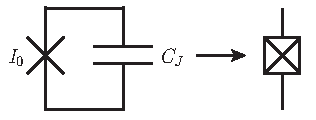
\includegraphics[width = 2.11in]{scqb_chapter/JJ_schem}
\end{center}
\caption[Josephson junction circuit schematic]{Circuit model for a Josephson junction including the intrinsic geometric parallel-plate capacitance.  The symbol at right is the circuit symbol for a junction including its intrinsic capacitance.}
\label{fig:JJ_schem}
\end{figure*}

From the definition of inductance $L = V/\dot{I}$ and equations (\ref{eq:CPR}) and (\ref{eq:2nd_JR}), we find that the impedance of the Josephson junction is that of an inductor whose value depends on the current flowing through it,
 \begin{equation}
L_J = \frac{\Phi_0}{2 \pi I_0 \cos{\delta}} = \frac{L_{J0}}{\sqrt{1 - I^2/I_0^2}}
\label{eq:LJ}
\end{equation}
where $L_{J0} = \Phi_0/2\pi I_0$ is the ``linear'' inductance of the junction for very small current.  For any physical Josephson junction, the thin metal-insulator-metal sandwich also forms an effective parallel-plate capacitor, usually modeled as an extra capacitance in parallel with the ideal Josephson element as shown in Figure \ref{fig:JJ_schem}.  Thus, a Josephson junction is itself intrinsically a nonlinear LC oscillator.  Due to the form of (\ref{eq:LJ}), the inductance of the junction increases with increasing current, and thus the resonant frequency of the Josephson nonlinear oscillator decreases.  For moderate excitations, this looks much like the softening potential drawn previously in Figure \ref{fig:anh_pot}b.

Because the critical current and the junction capacitance scale linearly with the area of the junction, the self-resonant frequency (also called the \textit{plasma frequency}) of the junction
\begin{equation}
\omega_J = \sqrt{\frac{2 \pi I_0}{\Phi_0 C}}
\label{eq:plas_freq}
\end{equation}
is fixed for a given junction fabrication process.  This frequency is typically many tens of gigahertz, and is usually reduced by adding an additional shunt capacitance in parallel with the junction to bring the plasma frequency down into the few gigahertz regime for convenience of operation.  The full form of the potential can be calculated by expressing the energy in the junction $U$ as the time integral of the voltage across the junction multiplied by the current.  Assuming zero initial energy at $t = - \infty$ and applying the Josephson relations, the junction energy can be calculated as \cite{slichterthesis}
\begin{equation}
U = E_J (1 - \cos{\delta})
\label{eq:E_J}
\end{equation}
where $E_J$ is the characteristic Josephson energy scale $E_J = \Phi_0 I_0/2\pi = \hbar I_0/2e$.  Thus, we see that the full potential is a cosine function with a characteristic scale determined by the junction critical current.

\subsection{Transmon qubits}

The circuit implementation of the anharmonic oscillator I described in the previous section is called a \textit{transmon} qubit \cite{Houck2009,transmontheory}.  This circuit design was created at Yale and has become the superconducting qubit of choice for many research efforts in the field, and for good reason.  The transmon is a straightforward device to design, fabricate, and control, and is conceptually easy to think about.  Furthermore, the transmon consistently achieves long coherence times in the 10 to 100 microsecond range \cite{PhysRevB.77.180502,Paik_3DT}, very long compared to 10 to 50 nanoseconds, the typical time required to do an arbitrary rotation of the qubit state \cite{PhysRevLett.102.090502}.

The circuit schematic for the transmon qubit is, remarkably, no different from that of a Josephson junction with intrinsic shunt capacitance; the main difference is the presence of an additional, large external shunting capacitance across the junction.  The purpose of this large capacitance is to reduce the single-electron charging energy associated with the total capacitance $E_C = e^2 / 2 C$.  This effectively flattens the dispersion of the energy eigenstates in the charge dimension, ensuring that the transmon qubit is essentially immune to dephasing due to charge noise.  To ensure the qubit is deep in this regime, we generally target $E_C$ to be about 1\% of $E_J$.  For an extensive theoretical discussion of the theory of the transmon, see reference \cite{transmontheory}.

The transition frequency between the two lowest energies of the transmon is approximately equal to the plasma frequency \eqref{eq:plas_freq}; re-expressing this in terms of $E_J$ and $E_C$ yields $\omega_{01} \approx \sqrt{8 E_J E_C}/\hbar$.  With the constraint $E_C \sim E_J/100$ and the requirement that the qubit frequency be experimentally convenient---say, 6 GHz---implies that $E_J \sim 3.5 \ \hbar \omega_{01} \sim h \times 20$ GHz, and thus $E_C \sim h \times 200$ MHz, with junction critical current $I_0 \sim 50$ nA and total capacitance $C \sim 100$ fF.  The primary limitation of the transmon qubit is the fact that the anharmonicity $\alpha$ is approximately $-E_C$, and thus the transition frequency $\omega_{12}$ is just a few percent lower than $\omega_{01}$.  To ensure that the transmon state remains in the $\{ \ket{0},\ket{1} \}$ manifold, the bandwidth of the control pulses used to induce qubit state transitions must be smaller than the anharmonicity \cite{PhysRevA.82.040305}.

\section{Cavity quantum electrodynamics}

With the transmon qubit in hand, we have a controllable, coherent quantum circuit with which we can perform experiments requiring a quantum two-level (or few-level) system.  However, we have not yet developed any description of how to couple these qubits to other quantum systems or to the outside world to enable the measurement of their quantum state.  In this section I will introduce the paradigm of \textit{cavity quantum electrodynamics} (cavity QED) \cite{bermanbook}, an approach which has been extremely fruitful in the study of real atoms \cite{RevModPhys.73.565,0034-4885-69-5-R02} and more recently quantum circuits \cite{cQEDtheory,blai07}.

\begin{figure*}
\begin{center}
	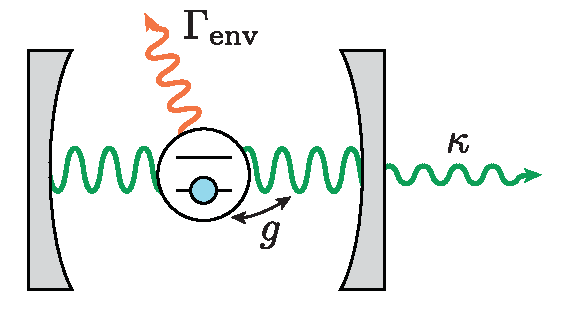
\includegraphics[width = 3.75in]{scqb_chapter/cav_QED}
\end{center}
\caption[Cavity QED schematic]{A simplified picture of a cavity QED setup.  An atom is placed inside a cavity resonator.  A particular transition of the atom is coupled to the standing mode inside the cavity with a coupling strength $g$.  The cavity filters the radiative density of states seen from the perspective of the atom, ideally reducing the atomic decay rate to the environment $\Gamma_{\rm env}$ to a negligible value.  One of the mirrors of the cavity is partially transmissive, allowing photons in the cavity mode to controllably leak out of the resonator at a rate $\kappa$.}
\label{fig:cav_QED}
\end{figure*}

A simplified picture of a cavity QED system is shown in Figure \ref{fig:cav_QED}.  The reasons for enveloping an atomic system of interest in a resonant cavity are several.  For atomic systems, perhaps most importantly, the presence of the cavity filters the radiative density of states seen by the atom.  A free excited atom in the continuum has a very large density of states to radiate into, and as a result atomic excited states tend to decay very quickly.  If the atomic transition of interest is tuned into resonance with the cavity, then the excited state will preferentially radiate into this mode.  However, because the resulting photon remains in the cavity for a long time, the atom has many opportunities to re-absorb it.  A more precise quantum picture of this process is simply that atomic excitation will be coherently exchanged with the resonator according to the coupling rate $g$.  If the coupling rate $g$ can be made much larger than the environmental decay rate $\Gamma_{\rm env}$ and the cavity decay rate $\kappa$, a cavity QED system can thus achieve strong coupling between a single atomic mode and a single photon, probing the most fundamental interaction diagrams in QED.

\subsection{Jaynes-Cummings Hamiltonian}

In the limit $\Gamma_{\rm env} \rightarrow 0$, and for now ignoring the cavity decay $\kappa$, a cavity QED system is described by the Hamiltonian \cite{wallbook}
\begin{align}
\label{eq:JC_H_terms} H & = H_q + H_r + H_{int} \\
& = \frac{1}{2}\hbar\omega_q\sigma_z + \hbar \omega_r a^{\dagger} a + \hbar g (a +a^{\dagger})(\sigma_+ + \sigma_-), 
\end{align}
where on the first line we have broken up the Hamiltonian into terms describing the free evolution of the qubit and resonator ($H_q$ and $H_r$, respectively) and their interaction ($H_{int}$), and $\omega_q$ is the transition frequency of the two-level atom, $\omega_r$ is the cavity resonant frequency, $a^{\dagger}$ and $a$ are the cavity creation and annihilation operators, and $\sigma_+$ and $\sigma_-$ are the qubit raising and lowering operators given by $(\sigma_x \pm i \sigma_y)/2$.  We can simplify this expression by ignoring the interaction terms that don't conserve excitation number (the ``rotating wave approximation''), resulting in the Jaynes-Cummings (JC) Hamiltonian
\begin{equation}
H_{JC} = \frac{1}{2}\hbar\omega_q\sigma_z + \hbar \omega_r a^\dagger a + \hbar g (a \sigma_+ +a^\dagger \sigma_-).
\label{eq:JC_H}
\end{equation}
The interaction term can now be interpreted in a straightforward manner as the exchange of an excitation between the atom and cavity.  The elegant simplicity of this Hamiltonian is one of the reasons for the remarkable success of cavity QED systems in implementing highly coherent control of single atomic quantum degrees of freedom.

\subsection{Circuit implementation of cavity quantum electrodynamics}

\begin{figure*}
\begin{center}
	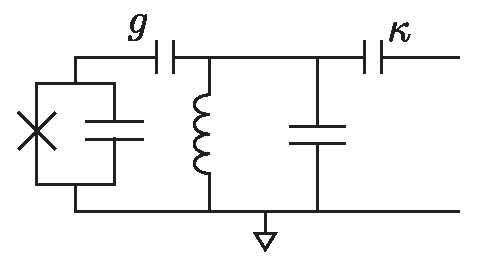
\includegraphics[width = 3.25in]{scqb_chapter/cQED}
\end{center}
\caption[Circuit QED schematic]{A circuit diagram which implements the same Hamiltonian as a cavity QED system.  A transmon qubit, at left, is capacitively coupled with strength $g$ to an LC resonator.  The resonator is capacitively coupled to the environment with rate $\kappa$.  It is also quite possible to replace one or both capacitive couplings with inductive couplings.  The circuit as drawn contains an explicit ground reference, though this is not necessary and cQED systems are often implemented as partially or fully differential circuits to reject common-mode interference.}
\label{fig:cQED}
\end{figure*}

I have already introduced all of the components necessary to realize an electrical circuit which is entirely analogous to a cavity QED system.  This paradigm is known as \textit{circuit QED} (cQED); a circuit schematic for such a system is shown in Figure \ref{fig:cQED}.  A superconducting transmon qubit plays the role of a single atom, and an electrical resonator plays the role of the cavity.  However, there are several important differences between atomic cavity QED and cQED.  Atomic systems are limited in the magnitude of $g$ by the size of the intrinsic dipole moment of the atomic transition of interest.  In circuit-based systems, $g$ can be adjusted independently of the other parameters by altering the size of the coupling capacitor, and schemes have even been demonstrated to dynamically tune this parameter on the same time scale as coherent qubit state rotations \cite{PhysRevB.84.184515}.

Additionally, circuits do not suffer from the intrinsic free-space radiative problem of real atoms, as they need not have any true geometric dipole moment.  Thus, for cQED systems, reduction of $\Gamma_{\rm env}$ is not a primary motivation for coupling the qubit to a cavity.  Furthermore, this also implies that the qubit need not be placed ``inside'' the cavity, permitting the use of flexible circuit topologies.  For cQED systems, the real reason for the cavity is to permit the non-invasive measurement of the qubit state, which is the subject of the next section.  In some multi-qubit experiments, several qubits are coupled to the same cavity which is then used as a ``quantum bus'' to allow the controllable coherent exchange of energy between the qubits \cite{Majer2007,Mariantoni2010}.

Although the system described so far is entirely composed of circuit elements, a experimentally practical hybrid system called the ''3D transmon'' architecture is commonly used as well \cite{Paik_3DT}.  The circuit comprising the transmon qubit is essentially the same, but rather than being capacitively-coupled to a circuit-style resonator, the qubit is coupled to a mode of a 3D waveguide cavity with a pair of large antenna paddles.  This architecture provides very long qubit coherence times by minimizing the interaction between the quantum modes of the qubit and any defects in the materials on which it is fabricated.  All of the experiments described in this thesis use this 3D transmon architecture.

\subsection{Dispersive regime and QND measurement}

Though the JC Hamiltonian generally describes the behavior of cQED systems for a large range of parameter regimes, the most relevant regime for the experiments described in this thesis is the so-called \textit{dispersive} regime, where the magnitude of the qubit-cavity detuning $\Delta = \omega_q - \omega_r$ is much larger than the coupling rate $g$.  Since excitations are quantized, in this regime the qubit and cavity cannot efficiently exchange energy with one another.  By expanding $H_{int}$ to second order in the small parameter $g/\Delta$ we find a revised interaction term
\begin{equation}
H_{int} =- \chi a^{\dagger} a \sigma_z
\end{equation}
where we've introduced the dispersive coupling rate $\chi = g^2 / \Delta$. Because $H_q \propto \sigma_z$ and $H_r \propto a^\dagger a$, the interaction term now commutes with the qubit and resonator terms, satisfying the requirement for a QND measurement (\ref{eq:QND_cond}).  This can be made more explicit by rewriting (\ref{eq:JC_H_terms}) with the dispersive interaction $H_{int}$ and re-grouping the terms as
\begin{equation}
H_{disp} = \frac{1}{2} \hbar \omega_q \sigma_z + \hbar \left(\omega_r + \chi \sigma_z \right)a^\dagger a.
\label{eq:Hdisp_qumeas}
\end{equation}
We can interpret the second term as the Hamiltonian of a quantum harmonic oscillator with a resonant frequency shifted by $\pm \chi$ depending on the qubit state operator $\sigma_z$.  Thus, a measurement which probes the resonant frequency of the cavity realizes a QND measurement of the state of the qubit.

Our choice of the grouping of the terms in (\ref{eq:Hdisp_qumeas}) was entirely arbitrary; we could have instead lumped the interaction term into $H_q$, realizing the Hamiltonian
\begin{equation}
H_{disp} = \frac{1}{2} \hbar (\omega_q + 2 \chi a^\dagger a)  \sigma_z + \hbar \omega_r a^\dagger a.
\label{eq:Hdisp_cavmeas}
\end{equation}
Now we can interpret the first term as a qubit whose transition frequency is shifted\footnote{This frequency shift can be interpreted as an incarnation of the AC Stark effect.} by $2 \chi$ times the photon number operator $a^\dagger a$, and thus a measurement which probes the transition frequency of the qubit realizes a QND measurement of the cavity photon number.  In reality, both of these effects occur simultaneously, and which form of the Hamiltonian we consider is largely a matter of convenience dictated by which quantity is measured in an experiment.  None of the experiments performed in this thesis involve the frequency-selective measurement of the qubit state, and thus I will focus the discussion to how measurement is performed within the context of (\ref{eq:Hdisp_qumeas}).

How is a measurement of the cavity frequency performed in practice?  A probe signal is injected into the cavity; this signal becomes entangled with the qubit state, and subsequently leaks out of the cavity at the rate $\kappa$.  A measurement of some property of this signal that differs for the two qubit states consumes the entanglement and delivers some information about that state.  Generally speaking, the signals used for measurement are coherent states, classically represented as a complex phasor $a e^{i \phi}$.   If the amplitude or phase of this vector differs between the two qubit states, a measurement of this quantity amounts to a measurement of the qubit state.  The details of this scheme depend on the parameter regime of the experimental realization.  For simplicity in this discussion I will only consider a cQED system measured in reflection \cite{Boissonneault2009,Girvin2014}, and I will also assume the cavity has no important internal losses.

\begin{figure*}
\begin{center}
	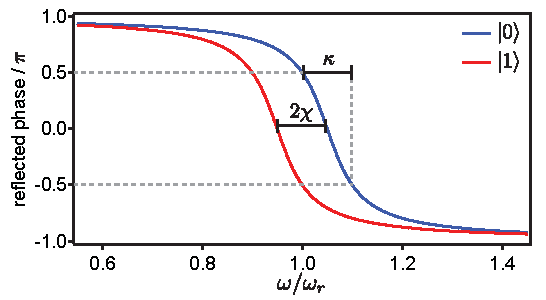
\includegraphics[width = 3.64in]{scqb_chapter/ref_phi}
\end{center}
\caption[Dispersive phase shift in reflection]{Reflected phase shift vs. normalized frequency for the case $2 \chi = \kappa$ where $\chi$ is negative.  Measuring the phase of a reflected probe signal at a frequency where the reflected phase differs constitutes a measurement of the state of the qubit.}
\label{fig:ref_phi}
\end{figure*}

When a cavity is measured in reflection, the probe signal acquires a frequency-dependent phase shift plotted in Figure \ref{fig:ref_phi}.  The total phase shift is zero at the resonant frequency $\omega_r$ and $\pm \pi$ at large detunings.  If the qubit is in the $\ket{0}$ ($\ket{1}$) state, the cavity resonance is shifted by $-\chi$ ($+\chi$).  Thus, a measurement signal at an intermediate frequency acquires a different reflected phase for the two states.  Whether or not this measurement constitutes a projective or partial measurement of the state depends on a variety of system parameters, including the magnitude of the coherent state $\bar{n}$, the amount of time the output signal is integrated for, and the magnitude of the phase shift.  For the case of a transmission measurement the picture is essentially the same, though the phase shift is reduced by a factor of 2 and the two signals will have a difference in amplitude as well as phase if the measurement frequency is not at exactly $\omega_r$.

\begin{figure*}
\begin{center}
	\includegraphics[width = 6in]{scqb_chapter/IQ_blobs.png}
\end{center}
\caption[IQ histograms for various parameters]{Simulated histograms for qubit-state-dependent IQ shifts.  The finite spatial extent of the histograms is due to quantum and classical noise in the two quadratures of the field.  \textbf{a} Well-separated histograms for $\Delta \theta = \pi/2$.  \textbf{b} Significantly overlapping histograms for the same coherent state amplitude, but with $\Delta \theta = \pi/6$.  \textbf{c} Increased histogram separation can be achieved for small phase shifts by increasing the coherent state amplitude.}
\label{fig:IQ_blobs}
\end{figure*}

For a single set of measurement parameters, we can qualitatively determine the strength of the measurement by plotting histograms of the measurement outcomes for the different qubit states in terms of the two cartesian coordinates (real and imaginary) which make up the complex phasor.  In the language of microwave electronics, these two coordinates are called the \textit{in-phase} and \textit{quadrature} components of the signal, or I and Q.  These histograms are depicted in Figure \ref{fig:IQ_blobs}.  For a single measurement, if the histograms are well-separated as in Figure \ref{fig:IQ_blobs}a, this constitutes a projective measurement of the qubit state (corresponding to Figure \ref{fig:ideal_proj_meas}).  If the histograms are significantly overlapping, we realize a partial measurement of the qubit state (corresponding to Figure \ref{fig:ideal_partial_meas}).  Keeping all other parameters fixed, we can increase the histogram separation by increasing the length of the coherent state vector.  However, there are practical limits to the maximum signal which can be utilized in a dispersive cQED measurement.  The dispersive approximation itself supplies a rough upper limit, as the validity of the dispersive approximation relies on the condition $\bar{n} < \bar{n}_{\textrm{crit}} = \Delta^2/4g^2$ \cite{slichterthesis}.  In practice this is not a hard limit, and relatively high-quality qubit readout has been performed with $\bar{n} \sim 3 \bar{n}_{\textrm{crit}}$ or so \cite{Jeffrey2014}.  At these large photon numbers, the measurement is typically no longer perfectly QND, but for short measurement times the error rate can be negligibly small.

It is important to note that because the transmon is only a weakly anharmonic system, the higher level transitions will also couple to the cavity mode, which significantly complicates the simple picture of a two-level system coupled to the cavity with a strength $g$.  The dispersive shift $\chi$ is no longer simply given as $g^2/\Delta$, but will rather be a sum over all of the coupling strengths $g_{ij}$ for the various state transitions $\omega_{ij}$.  For the experiments conducted in this thesis, this additional complexity can be entirely absorbed as a rescaling of the circuit QED parameters; in general the coupling strength $g$ is not directly important, and the dispersive shift $\chi_{01}$ due to the first level transition is directly measured in experiment anyway.  For a full treatment of the multi-level transmon in circuit QED, see references \cite{slichterthesis,Weber2014a}.

\subsection{Back-action of cQED measurement}\label{s:cQED_backaction}

Most of the results in this thesis were made with cQED systems in the dispersive weak measurement limit.  As discussed previously, the strength of a measurement depends not only on the fixed system parameters but also on the signal magnitude used in the measurement; thus, a vast range of measurement strengths can be accessed in a single apparatus.  However, the fixed system parameters result in a intrinsic scale of measurement strength corresponding to the state-dependent phase shift $\Delta \theta = 2 \tan^{-1}(2 \chi / \kappa)$, and several equations of interest take on a relatively intuitive and simple form in the limit $\Delta \theta \ll 1$.

To elucidate some of the interesting and unintuitive details of the back-action of the cQED measurement, I will follow the very good discussion in reference \cite{koro11}.  For a cQED setup in the dispersive limit with $\omega = \omega_r$, the ensemble dephasing due to the presence of a measurement coherent state with mean photon number $\bar{n}$ is given by
\begin{equation}
\Gamma = \frac{8 \chi^2 \bar{n}}{\kappa}.
\label{eq:cQED_dephasing}
\end{equation}
This coherent state corresponds to the oscillation of the field expectation value $\xpec{F(t)} = 2 \sqrt{\bar{n}} \sigma_{\rm gr} \cos(\omega t)$, where $\sigma_{\rm gr}$ is the ground state amplitude width due to quantum fluctuations which here serves to re-scale the coherent state amplitude into ``uncertainty units'' (note that $\sigma_{\rm gr} = 1/4$).  Interaction with the qubit then creates a phase shift of $\pm 2 \chi/\kappa$ depending on the qubit state.  Decomposing the resulting phasor into quadrature components results in
\begin{gather}
\xpec{F(t)} = \rm I \cos(\omega t) + \rm Q \sin(\omega t) \notag \\
\rm I = 2 \sqrt{\bar{n}} \sigma_{\rm gr} \quad \rm Q = 2 \sqrt{\bar{n}} \sigma_{\rm gr} (2 \chi / \kappa) \xpec{\sigma_z}
\end{gather}
We can now explicitly see the information contained in each quadrature.  The large I quadrature contains information about the photon number fluctuations in the resonator, while the small Q quadrature contains information about the qubit state.  If we use an interferometric apparatus to selectively measure only the Q quadrature (this will be a phase-sensitive parametric amplifier; see section \ref{s:phase_sens_amps}), by emptying the resonator of its contents we can measure the Q quadrature with imprecision $\sigma_{\rm gr}$.  In the limit of a continuous-time measurement, we achieve an imprecision in Q of $\sigma_{\rm gr} / \sqrt{\kappa t}$, or, equivalently, an imprecision in $\xpec{\sigma_z}$ of $\sqrt{\kappa/t}/(4 \chi \sqrt{\bar{n}})$.  Linking back to the discussion in section \ref{s:bayesian}, the full swing of our detector between $\sigma_z = \pm 1$ is thus
\begin{equation}
\Delta V = 8 (\chi/\kappa) \sqrt{\bar{n}} \sigma_{\rm gr},
\end{equation}
and the imprecision $\sigma$ in the output signal $V(t)$ is
\begin{equation}
\sigma = \sqrt{\frac{\kappa}{t}} \left( \frac{\Delta V}{8 \chi \sqrt{\bar{n}}} \right).
\end{equation}
Thus, we can express the power spectral density of the output noise as
\begin{equation}
S = 2 t \sigma^2 = \frac{ (\Delta V)^2 \kappa}{32 \chi^2 \bar{n}}.
\end{equation}
From \eqref{eq:bayesian_dephasing}, we calculate the dephasing rate associated with this measurement as
\begin{equation}
\Gamma = \frac{(\Delta V)^2}{4S} = \frac{8 \chi^2 \bar{n}}{\kappa}.
\end{equation}

This is an important result; because the dephasing rate associated with measuring only the Q quadrature of the output signal accounts for all of the ensemble qubit state dephasing, this measurement process can have no back-action besides the Bayesian evolution described in section \ref{s:bayesian}.  Thus, the only back-action of this measurement process is the stochastic evolution of the Bloch vector towards one of the poles, with no accompanying evolution in the phase of an initial superposition.  In other words, if the Bloch vector begins on a particular meridian of the Bloch sphere, the action of the measurement is to drive stochastic evolution of the state vector along this meridian only.

What if we were to instead measure the I quadrature?  For a measurement time $t$, we measure I with an imprecision $\sigma_{\rm gr} / \sqrt{\kappa t}$, which can be understood as a measurement of the fluctuation of the number $N$ of emitted photons in that time $\mathrm{var}(N) = \bar{n}\kappa t$, which follows from the fact that the variance of the photon number in a coherent state is equal to the mean photon number $\bar{n}$, the photons are leaking from the cavity at the rate $\kappa$, and we capture them for a time $t$.  Because the correlation function of photon number in the resonator depends on time as $\exp(-\kappa t/2)$ \cite{clerk_revmod}, the effect of detecting an amplitude fluctuation corresponding to one photon\footnote{Because our detector output is a continuous field variable and not a photon-counting detector, thinking of the output field in terms of individual photon detection events is not formally correct, but the intuition it provides is essentially correct if we're careful about factors of 2.} implies that that fluctuation on average spent a time $2/\kappa$ in the resonator (this is the lifetime of the field amplitude; the power of course has the lifetime $1/\kappa$), resulting in an evolution of the qubit phase by $4\chi/\kappa$.  Thus, the variance in the qubit phase is $\mathrm{var}(\phi) = (4 \chi/\kappa)^2 \bar{n}\kappa t$, implying a dephasing rate $\Gamma = \mathrm{var}(\phi) / 2 t = 8\chi^2 \bar{n} / \kappa$.  We have once again recovered the standard result for the total ensemble dephasing, implying that the resulting ``pure dephasing'' associated with measuring the I quadrature represents the entire back-action of the measurement.

What if we were to measure both the I and Q quadratures simultaneously?  The measurement simultaneously acquires information about both the qubit state and the photon number fluctuations, and both kinds of back-action occur simultaneously.  It turns out (see section \ref{s:phase_pres_amps}) that due to the field commutation relations, an ideal measurement of both quadratures implies doubling the size of the uncertainty compared to the single-quadrature case.  Because the power spectral density of the noise has been increased by a factor of two, the dephasing rate for each back-action process is reduced by a factor of two, both then contributing an equal half of the total dephasing rate $\Gamma$ in \eqref{eq:cQED_dephasing}.  An in-depth discussion of how both single-quadrature and two-quadrature measurements are made in practice is the subject of the next chapter.































